% sec2.tex — c02｜原文 p6–p12，并含 p13 上半的 §2 尾部（例 2.22 的式 (20) 及注 2.23、例 2.24）
% 公式号 (6)–(20)；编号环境 2.1–2.24
% 块边界：从 p6 底部 "2. The homotopy type of quantum mechanics" 标题下的正文起（\section 本体在 main.tex）；
% p6 顶部的 §1.4–§1.5 由 sec1.tex 完成，本块不重复。本块终于例 2.24（§2 结束），§3 的标题在 main.tex。

% [原文 p.6]
设 $M$ 是闭的定向 Riemann 流形。$M$ 上的经典力学研究路径 $x\colon I\to M$，其作用量泛函为 $S(x)=\frac{1}{2}\int_I\|\dot{x}\|\,dt$。$S$ 的临界点是 $M$ 中参数化的测地线。利用指数映射与度量，这样的测地线可以与 $M$ 的余切丛等同起来。辛流形 $T^{*}M$ 的量子化产生 $M$ 上的量子力学，例如参见 [BW97]。下文只要求量子化的两项基本输出：(i) 状态空间 $\cH=L^{2}(M)$，以及 (ii) 由 $M$ 上的拉普拉斯算子给出的哈密顿量 $H=\Delta$。在 Wick 转动后的量子力学中，$(\cH,H)$
% [Tutor Note: 此处 $S$ 是长度泛函（原文未平方），其临界点即参数化测地线；若改用能量泛函 $\frac12\int_I\|\dot{x}\|^{2}dt$，临界点是常速测地线。核对时勿按能量泛函自行补平方。]

% [原文 p.7]
确定半群 $(\R_{\ge 0},+)$ 的一个表示
\begin{equation}
\R_{\ge 0}\to\mathrm{End}(\cH),\qquad t\mapsto e^{-tH}
\tag{6}
\end{equation}
取值于 $\cH$ 上的自伴算子，且当 $t>0$ 时为迹类（这里用到 $M$ 的紧性）。这引出下面的定义，其精确表述将在下文 §2.1 给出。
% [Tutor Note: (6) 中 $e^{-tH}$ 与后文 (11) 的 $E(\mathrm{I}^{\pm}_t)=e^{-tH}$ 是同一个半群；$t>0$ 的迹类条件正是配分函数 $\Tr(e^{-tH})$（式 (11) 中 $E(S_t)$）收敛所需的，核对 (11) 第三行。]

\begin{definition}[2.1]
一个\emph{量子力学系统}是一个状态空间 $\cH$ 与一个哈密顿量 $H$，它们确定一个自伴的、迹类的表示 (6)。量子力学系统 $(\cH,H)$ 与 $(\cH',H')$ 称为\emph{等价的}，若存在酉映射 $u\colon\cH\to\cH'$ 使得 $H'=uHu^{-1}$。
\end{definition}
% [Tutor Note: 等价条件原文写作 $H'=uHu^{-1}$（即 $H'u=uH$），不是 $u^{-1}Hu$；这与“$u$ 把 $H$ 的算子搬到 $\cH'$ 上”的约定一致，抄写时勿随手改序。]

本节的目的是把量子力学系统及其等价组装成一个拓扑群胚，即一个叠。这个叠的基本特征可以推广到与猜想 1.1 相关的更精细的物理理论。事实上，关于猜想 1.1 的许多直观都源自对量子力学中各项结构的展开。

\begin{remark}[2.2]
定义 2.1 有几处变体。放弃迹类条件会导向\emph{非紧的}理论；例子包括非紧流形上的量子力学。放弃自伴条件会导向非酉理论的 Wick 转动。尽管完整的图景尚未被完全理解，这些例子提示：与猜想 1.1 相关的正是（Wick 转动后的）紧的、酉的量子理论。
\end{remark}

\subsection{量子力学理论的空间是 $K(\Z,3)$}
定义 2.1 中的哈密顿量是一类自伴无界算子\footnote{$\cH$ 上的\emph{无界算子}是指一个定义域 $\mathrm{dom}(H)\subset\cH$ 与一个线性映射 $H\colon\mathrm{dom}(H)\to\cH$。无界算子称为\emph{自伴的}，若它在其定义域的闭包上自伴。}，它们可以用构形空间给出几何描述 [HST10, §4]。简言之，给定一个自伴无界算子 $H$，一族两两正交的特征子空间 $\{\cH_\lambda\subset\cH\}_{\lambda\in\R}$ 决定 $\R$ 上的一个构形，其中 $\lambda\in\R$ 被特征子空间 $\cH_\lambda\subset\cH$ 标记；见图 1。反之，给定 $\R$ 上的一个构形，定义其定义域为 $\bigoplus_{\lambda\in\R}\cH_\lambda$ 的无界算子，其中 $H\colon\bigoplus_{\lambda\in\R}\cH_\lambda\to\cH$ 是在 $\cH_\lambda$ 上乘以 $\lambda$ 的线性映射。
% [Tutor Note: 原文第 3 号脚注。译文用 LaTeX 自动脚注，编号可能与原文不同，核对时以“无界算子+自伴”这条注释为准。]

无界算子上的拓扑决定构形上的拓扑：一对构形称为接近的，若存在（能量截断）$\Lambda\in\R$ 使得特征值 $\lambda<\Lambda$ 的那些特征子空间接近；这一拓扑的精确定义参见 [HST10, Definition 4.3, Proposition 4.4]。一个无界算子 $H$ 在其定义域的闭包上给出半群表示 (6)，我们再把它在定义域的正交补上用零映射延拓 [HST10, Proposition 5.9]。要使半群表示是迹类的，必须对 $H$ 附加要求：非零的标号 $\lambda\in\R$ 有下界，每个子空间 $\cH_\lambda\subset\cH$ 有限维，谱 $\Spec(H)\subset\R$ 离散，且 $\lambda$ 满足某些增长条件。细节参见 [HST10, §3]。

\begin{definition}[2.3]
\emph{哈密顿量的空间}，记作 $\Ham$，是构形 $\{\cH_\lambda\subset\cH\}_{\lambda\in\R}$ 构成的空间，这些构形决定生成迹类自伴半群表示 (6) 的无界算子。
\end{definition}

酉群 $\mathrm{U}(\cH)$ 通过共轭作用在无界算子上，这给出 $\mathrm{U}(\cH)$（带紧开拓扑）在 $\Ham$ 上的连续作用。\footnote{连续性来自 $\Ham$ 中开子集的描述 [HST10, Definition 4.3]，以及 $\mathrm{U}(\cH)$ 在紧算子上的作用的连续性，参见 [AS04, Proposition A1.1] 与 [EU14]。}这一共轭作用经过标量商 $\mathrm{PU}(\cH)=\mathrm{U}(\cH)/\mathrm{U}(1)$ 分解。
% [Tutor Note: 原文第 4 号脚注。“连续性”指作用 $\mathrm{U}(\cH)\times\Ham\to\Ham$ 连续；原文给出的两条依据分别是 $\Ham$ 上的拓扑（开子集描述）与紧算子拓扑下的连续性。]

\begin{definition}[2.4]
定义拓扑范畴 $\QM:=\Ham/\!/\mathrm{PU}(\cH)$ 为由酉群的共轭作用所诱导的作用的商群胚（quotient groupoid）。
\end{definition}

我们强调，并不要求无界算子的定义域在 $\cH$ 中稠密。因此，定义 2.3 不要求包含 $\bigoplus_{\lambda\in\R}\cH_\lambda\subset\cH$ 是稠密的。

\begin{example}[2.5（拓扑场论）]
任何子空间 $V\subset\cH$ 定义一个无界算子 $T_V$，其 $\mathrm{dom}(T_V)=V$，线性映射为零映射 $T_V\equiv 0\colon V\to\cH$。这一无界算子确定 $\Ham$ 中一个点，当且仅当 $V$ 是有限维的。相应的量子系统是\emph{拓扑的}，其构形为支撑在 $0\in\R$ 的 $\cH_0=V$。注意时间演化 (6) 在 $t$ 中是常值的：没有动力学。假设 2.14 把它与 Atiyah 的拓扑场论定义相比较。
\end{example}

% [原文 p.8]
\figomit{1}{左图是构形空间模型中的一个哈密顿量，其中每个标记 $\cH_\lambda\subset\cH$（$\lambda\in\R$）是 $H$ 的、特征值为 $\lambda$ 的特征子空间。当标记相撞时，子空间相加。能量也可以「逃逸」到无穷远。右侧的图沿用 [Wit82a] 的记号：每个特征子空间的维数由 $\circ$ 的个数（状态数）记录。这些维数把构形确定到同构为止。如虚线箭头所示，标记相撞会使维数相加。}
% [Tutor Note: 原文图注末句 "colliding labels adds dimensions" 主谓不一致（colliding labels 为复数，应为 add）；译文按正确语法处理，已登记 ERRATA。]
% [Tutor Note: 原文中图 1 是浮动体，排在 p8 顶端，把例 2.5 的末句割到图后；译文按原排版位置把图放在例 2.5 之后、注 2.6 之前，句序不变。]

\begin{remark}[2.6]
群胚 $\QM$ 中的对象以及它们在图 1 中的描绘，在量子力学中有如下解释。对 $\QM$ 中的一个对象，特征子空间 $\cH_\lambda$ 对应能量为 $\lambda$ 的状态。$\QM$ 的对象上的拓扑允许能量值发生扰动，也允许能量特征子空间的分裂与合并。特征值最小的那个特征子空间包含理论的\emph{基态}。当 $H$ 的定义域 $\mathrm{dom}(H)\subset\cH$ 不稠密时，闭包的补 $\ol{\mathrm{dom}(H)}^{\perp}$ 是「无穷远处」的特征子空间，即无穷能量的状态。从这一观点看，也许最好把理论的真正状态空间看作有限能量特征态的闭包 $\bigoplus_{\lambda<\infty}\cH_\lambda\subset\cH$。以这一观点，拓扑理论的状态空间完全由基态组成。
\end{remark}
% [Tutor Note: 若 $\mathrm{dom}(H)$ 不稠密，则由 (6) 的零延拓，$\ol{\mathrm{dom}(H)}^{\perp}$ 上的演化为 $0$，故这些态对应“能量无穷”的极限；对照例 2.5 中 $V$ 支撑在 $0$ 的图景（那里 $\mathrm{dom}$ 的补恰为无穷能量的部分）。]

\begin{proposition}[2.7（{[HST10, §6]} {[ST04, §3.1]}）]
当 $\cH$ 是无穷维可分 Hilbert 空间时，$\QM$ 的几何实现是 Eilenberg–MacLane 空间
\begin{equation}
|\QM|\simeq K(\Z,3).
\tag{7}
\end{equation}
\end{proposition}

\begin{proof}[证明梗概]
哈密顿量空间的可缩性是 [HST10, Theorem 6.35]。简言之，$\Ham$ 有一个由定义域为 $\{0\}$ 的无界算子给出的基点。存在到该基点的收缩同伦，它把所有特征子空间一致地推到无穷远，从而使哈密顿量形变。于是 $|\QM|\simeq|\mathrm{pt}/\!/\mathrm{PU}(\cH)|\simeq\BPU(H)$。
% [Tutor Note: 原文此处先写 $\BPU(H)$（斜体 $H$），下一段又写 $\BPU(\cH)$（花体 $\cH$），记号不一致；两处均指 $\mathrm{PU}(\cH)$ 的分类空间，照原样排。]

其次，我们断言 $\mathrm{U}(\cH)$ 可缩；在范数拓扑下这是 Kuiper 的经典结果 [Kui65]，在紧开拓扑下这是 [AS04, Proposition A2.1]。利用纤维序列 $\mathrm{U}(1)\to\mathrm{U}(\cH)\to\mathrm{PU}(\cH)$ 计算 $\pi_*\mathrm{PU}(\cH)$，得到 $\BPU(\cH)\simeq BK(\Z,2)\simeq K(\Z,3)$。
% [Tutor Note: 补出省略的论证：$\mathrm{U}(\cH)$ 可缩给出 $\mathrm{PU}(\cH)\simeq B\mathrm{U}(1)=K(\Z,2)$（由纤维序列的长正合列 $\pi_1\mathrm{U}(1)\cong\pi_2\mathrm{PU}(\cH)$ 等），再取分类空间得 $\BPU(\cH)\simeq K(\Z,3)$。]
\end{proof}

分类空间 (7) 捕捉量子力学的同伦内容，但更精细的信息来自对叠 $\QM$ 的细致分析。下面简述与紧 Lie 群的射影表示的联系。

\begin{definition}[2.8]
设 $G$ 是紧 Lie 群。\emph{带 $G$-对称性的量子力学系统}构成的叠是映射叠（mapping stack）$\mathrm{Map}(\mathrm{pt}/\!/G,\QM)$。
\end{definition}

为展开这一定义，$\mathrm{Map}(\mathrm{pt}/\!/G,\QM)$ 中的一个对象（即叠的映射 $\mathrm{pt}/\!/G\to\QM$ 的数据）是 $\Ham$ 中一个点 $H$ 连同同态 $\alpha\colon G\to\mathrm{PU}(\cH)$
% [原文 p.9]
满足一个相容性条件。为陈述这一相容性，拉回
\begin{equation}
\begin{array}{ccccccccc}
1 & \longrightarrow & \mathrm{U}(1) & \longrightarrow & G^{\alpha} & \longrightarrow & G & \longrightarrow & 1\\[3pt]
 & & {\scriptstyle=}\big\downarrow & & \big\downarrow & \lrcorner & \big\downarrow{\scriptstyle\alpha} & & \\[3pt]
1 & \longrightarrow & \mathrm{U}(1) & \longrightarrow & \mathrm{U}(\cH) & \longrightarrow & \mathrm{PU}(\cH) & \longrightarrow & 1
\end{array}
\tag{8}
\end{equation}
决定 $G$ 的一个中心扩张（central extension）$G^{\alpha}$ 以及 $\cH$ 上的一个酉 $G^{\alpha}$-表示。$\alpha$ 与 $H$ 之间的相容性条件是：$\cH$ 上的 $G^{\alpha}$-作用与 $H$ 交换。
% [Tutor Note: (8) 中 $\lrcorner$ 表示方块是拉回：$G^{\alpha}=G\times_{\mathrm{PU}(\cH)}\mathrm{U}(\cH)$，其中右竖直箭头是 $\alpha$、左竖直箭头是相等（$\mathrm{U}(1)$ 不动）。这正是“$\alpha$ 的中心扩张由拉回得到”的含义。]

\begin{remark}[2.9]
带 $G$-对称性的量子系统增强图 1 中的构形：每个 $\cH_\lambda\subset\cH$ 是一个有限维 $G^{\alpha}$-表示，而构形中相撞的点对应表示的直和。
\end{remark}

\begin{example}[2.10（$G$-流形上的量子力学）]
设 $M$ 是定向紧 Riemann 流形，带有等距且保向的 $G$-作用。那么本节开头讨论的例子继承额外的结构：$\cH=L^{2}(M)$ 获得一个与哈密顿量 $H=\Delta$ 交换的 $G$-作用。这给出映射
\[
\mathrm{pt}/\!/G\to\Ham/\!/\mathrm{U}(\cH)\twoheadrightarrow\Ham/\!/\mathrm{PU}(\cH)=\QM
\]
它定义一个带（非射影）$G$-对称性的量子系统。
\end{example}

\begin{example}[2.11（自由费米子）]
在 1 维，$n$ 个\emph{自由费米子}的经典理论有场与作用量泛函
\begin{equation}
\psi\colon\R\to\R^{n},\qquad S(\psi)=\frac{1}{2}\int_{\R}\langle\psi,\partial_t\psi\rangle\,dt
\tag{9}
\end{equation}
其中 $\langle-,-\rangle$ 是 $\R^{n}$ 上的标准内积。经典解是到 $\R^{n}$ 的常值映射。把 $\R^{n}$ 视为纯奇的向量空间，就用 $\R^{n}$ 上的标准内积给这些经典解赋予一个奇辛结构。量子化等价于构造 $\mathrm{Cl}_n$ 上的一个不可约模 $V$ [DEF+99, pg. 623]，它定义（量子）自由费米子的状态空间。由于经典解是常值映射（即没有动力学），哈密顿量为 $H\equiv 0$，于是该量子理论是拓扑的。正交群 $\mathrm{O}_n$ 通过代数同构作用在 Clifford 代数 $\mathrm{Cl}_n$ 上。用这个代数同构扭转 $V$ 上的 $\mathrm{Cl}_n$-作用，就对 $\mathrm{O}_n$ 的每个元素产生一个不可约 $\mathrm{Cl}_n$-模。由 Schur 引理，这决定 $V$ 上的一个射影 $\mathrm{O}_n$-作用。当 $n$ 为偶数时，$\Lambda^{\bullet}\C^{n/2}$ 是唯一的（分次的）不可约 $\mathrm{Cl}_n$-模，它作为 Fock 空间构造 [ST04, Definition 2.2.4]。在选定一个等距嵌入 $V\subset\cH$（这类嵌入构成的空间可缩）之后，自由费米子确定一个映射
\begin{equation}
\mathrm{pt}/\!/\mathrm{O}_n\to\QM
\tag{10}
\end{equation}
其相伴的中心扩张 (8) 为 $1\to\mathrm{U}(1)\to\mathrm{Pin}^{c}_{n}\to\mathrm{O}_n\to 1$。因此，自由费米子确定一个带（射影）$\mathrm{O}_n$-对称性的拓扑量子理论。
\end{example}
% [Tutor Note: $\mathrm{Pin}^{c}_{n}$ 是 $\mathrm{O}_n$ 被 $\mathrm{U}(1)$ 的中心扩张，正是 (8) 中 $G^{\alpha}$ 取 $G=\mathrm{O}_n$ 的情形；核对 (8) 与 (10) 的下标 $n$ 一致。]

\begin{remark}[2.12]
上述对自由费米子的描述没有反映 Clifford 代数与 Clifford 模上（重要的）$\Z/2$-分次。我们在例 2.24 中补救这一点。
\end{remark}

\subsection{量子系统作为配边范畴的表示}
特殊化定义 1.5，以 $\EBord_1$ 记\emph{1 维欧几里得配边范畴}。对象是 $\bullet=\mathrm{pt}^{+}$ 与 $\circ=\mathrm{pt}^{-}$ 的有限不交并，即点连同其定向的两种选择。态射是带边界的紧定向 1 维 Riemann 配边。人们发现（例如用 Morse 理论），这类配边是图 2 中那些配边的不交并。
配边通过沿匹配的源与靶数据粘接而复合。0 维与 1 维流形的不交并给范畴 $\EBord_1$ 赋予对称幺半结构。配边的复合引入关系，例如对 $s,t\in\R_{\ge 0}$，$\mathrm{I}^{\pm}_s\circ\mathrm{I}^{\pm}_t\simeq\mathrm{I}^{\pm}_{s+t}$ 对应区间长度相加这一事实，给出 (6) 中半群 $\R_{\ge 0}$ 的几何对应物。其他关系同样可以从图中读出。一个稍有不同的关系用到对称同构 $\sigma\colon\mathrm{pt}^{+}\sqcup\mathrm{pt}^{-}\xrightarrow{\ \sim\ }\mathrm{pt}^{-}\sqcup\mathrm{pt}^{+}$，它给出 $\sigma\circ\cap^{\pm}_t\simeq\cap^{\mp}_t$ 与 $\cup^{\pm}_t\circ\sigma\simeq\cup^{\mp}_t$。
% [Tutor Note: 这里的 $\cap$ 与 $\cup$ 是配边的图形名（“帽”与“杯”），不是集合运算；$\cap^{\pm}_t$ 表示半圆的两端分别为“上”与“下”，故定向反转把 $\pm$ 换成 $\mp$。核对图 2 与 (12)。]

% [原文 p.10]
\figomit{2}{$\EBord_1$ 中的态射是上述生成元的有限不交并。1 维流形 $S_t$ 是周长为 $t$ 的圆周，看作从空集到自身的配边。配边 $\mathrm{I}^{\pm}_t$、$\cup^{\pm}_t$ 与 $\cap^{\pm}_t$ 底下的 1 维流形都是长为 $t$ 的区间；它们之间的区别来自定向（由 $+$ 或 $-$ 表示）连同源与靶的数据。我们采用自下而上读配边的约定，例如 $\cap^{+}_t$ 的源是 $\mathrm{pt}^{-}\sqcup\mathrm{pt}^{+}$。}

密切相关的无定向 Riemann 配边范畴的一组完备生成元与关系见 [HST10, Theorem 6.11]，另见 [ST04, Proof of Proposition 3.1.1]。

一个定义 2.1 意义下的量子力学系统确定一个（非扭的）场论，取值为
\begin{equation}
\begin{array}{l}
E\colon\EBord_1\to\Vect,\qquad\qquad
\begin{array}{l}
E(\mathrm{pt}^{+})=V,\ E(\mathrm{pt}^{-})=\ol{V},\ E(\mathrm{I}^{\pm}_t)=e^{-tH},\\[2pt]
E(\cap^{+}_t)=\langle-,e^{-tH}-\rangle,\ E(S_t)=\Tr(e^{-tH})\\[2pt]
E(\cup^{+})\colon\C\to\ol{V}\otimes V\hookrightarrow\mathrm{End}(V),\ E(\cup^{+})(1)=e^{-tH}
\end{array}
\end{array}
\tag{11}
\end{equation}
其中 $V:=\mathrm{dom}(H)\subset\cH$ 是 $H$ 的定义域。反之，对称幺半函子 $E$ 的取值 $E(\mathrm{I}^{+}_t)$ 确定半群表示 (6)。为保证 $E(\mathrm{I}^{+}_t)$ 取值于自伴算子（从而确定一个量子力学系统），必须施加反射正性。为在当下框架中解释这些数据与结构，取 $\EBord_1$ 上由 1 维流形的定向反转生成的 $\Z/2$-作用。在图 2 的生成元上，定向反转是
% [Tutor Note: (11) 末两处写作 $E(\cup^{+})$，比生成元 $\cup^{\pm}_t$ 少了下标 $t$（原文如此，与 $E(\cap^{+}_t)$ 不对称）；下文 (19)、(20) 一律带 $t$。照原样排，勿自行补下标。]
\begin{equation}
\mathrm{pt}^{\pm}\mapsto\mathrm{pt}^{\mp},\qquad
\mathrm{I}^{\pm}_t\mapsto\mathrm{I}^{\mp}_t,\qquad
\cup^{\pm}_t\mapsto\cup^{\mp}_t,\qquad
\cap^{\pm}_t\mapsto\cap^{\mp}_t.
\tag{12}
\end{equation}
物理上，这个作用反转时间之箭。我们还有由复共轭生成的向量空间上的 $\Z/2$-作用。

\begin{definition}[2.13（反射正性，略述）]
函子 (11) 的一个\emph{反射结构}（reflection structure）是关于由定向反转与复共轭生成的 $\Z/2$-作用的等变数据，其中包含一个对合同构
\begin{equation}
E(\mathrm{pt}^{+})\xrightarrow{\ \sim\ }\ol{E(\mathrm{pt}^{-})}
\tag{13}
\end{equation}
的数据。带反射结构的表示 (11) 称为\emph{反射正的}，若 Hermite 配对
\begin{equation}
\langle-,-\rangle\colon\ol{E(\mathrm{pt}^{+})}\otimes E(\mathrm{pt}^{+})\simeq E(\mathrm{pt}^{-})\otimes E(\mathrm{pt}^{+})\xrightarrow{\ E(\cap^{-}_0)\ }\C
\tag{14}
\end{equation}
是正的。上式中，$\cap^{-}_0$ 是 $\cap^{-}_t$ 的 $t\to 0$ 极限。
\end{definition}
% [Tutor Note: (13) 的共轭落在 $\ol{E(\mathrm{pt}^{-})}$ 上，(14) 的共轭落在第一个因子 $\ol{E(\mathrm{pt}^{+})}$ 上，而 (15) 的共轭又回到 $\ol{E(\mathrm{pt}^{+})}$；三处取共轭的位置不同，抄写时按图核对，勿统一。]
% [Tutor Note: (14) 用到的同构 $\ol{E(\mathrm{pt}^{+})}\simeq E(\mathrm{pt}^{-})$ 正是 (13)；$\cap^{-}_0$ 是“半圆”退化为点的极限，故 (14) 就是 $V$ 上的内积，反射正性即该内积正定。]

按定义 1.9，(11) 与 (13) 是群胚 $\QFT_1:=\QFT^{1}_{1}(\mathrm{pt})$ 中一个对象的数据，该群胚由 $\cX=\mathrm{pt}$ 上的非扭 1 维欧几里得场论构成。

\begin{hypothesis}[2.14（比较 {[ST04, Definition 3.2.10]} 与 {[HST10, Corollary 6.28]}）]
存在叠的满态射 $\QFT_1\to\QM$，把定义 1.9 意义下的 1 维欧几里得场论送到定义 2.4 意义下的量子力学系统。
\end{hypothesis}

\begin{proof}[略证]
在对象上，叠的映射从对象 $E\in\QFT_1$ 出发，经由 $E(\mathrm{I}^{+}_t)$ 与（一个选定的）等距嵌入 $E(\mathrm{pt}^{+})\subset\cH$ 提取出半群表示。平凡扭场论之间的同构决定一个可逆的 $\C$-$\C$ 双模（即复直线）$L$ 以及预 Hilbert 空间之间的酉映射 $L\otimes E(\mathrm{spt}^{+})\to E'(\mathrm{spt}^{+})$ [ST11, §5.1]。这样的数据由预 Hilbert 空间的射影同构决定，而后者延拓为元素 $u\in\mathrm{PU}(\cH)$。这就完成了函子 $\QFT_1\to\QM$ 的梗概。

% [原文 p.11]
{\sloppy
要说明这个函子是满态射，基本想法是把图 2 中的图景提升为 $\EBord_1$ 的生成元与关系表现（比较 [HST10, Theorem 6.23]）。这样的表现表明，1 维欧几里得场论由内积空间 $(E(\mathrm{pt}^{+}),\langle-,-\rangle)$ 与由 $E(\mathrm{I}^{+}_t)$ 决定的自伴半群表示所决定。由 [HST10, Lemma 5.10]，有 $E(\mathrm{I}^{+}_t)=e^{-tH}$，其中 $H$ 是定义域为 $E(\mathrm{pt}^{+})\subset\cH$ 的唯一确定的无界算子。构造 (11) 于是给出 $\QFT_1\to\QM$ 的一个单侧逆。\par}
% [Tutor Note: 上文的 $\mathrm{spt}^{+}$ 与 (11) 中的 $\mathrm{pt}^{+}$ 是同一对象（ST11 的记号），故 $L\otimes E(\mathrm{spt}^{+})\to E'(\mathrm{spt}^{+})$ 就是把 (11) 的值经复直线扭一下后的同构。]
\end{proof}

\begin{remark}[2.15]
人们或许希望映射 $\QFT_1\to\QM$ 是等价，但这是不可能的：不同的拓扑内积空间（对应非同构的函子 (11)）可以有相同的 Hilbert 完备化。我们在注 3.21 中进一步讨论。
\end{remark}

\begin{corollary}[2.16]
例 2.5 意义下的拓扑理论对应 Atiyah 意义下的 1 维 Hermite 拓扑理论 [Ati89]。
\end{corollary}

\begin{proof}
在假设 2.14 的函子下，由有限维子空间 $V\subset\cH$ 与零哈密顿量确定的量子力学系统，对应由有限维内积空间 $V$ 与 $E(\mathrm{I}^{+})=\id$ 确定的 1 维场论。这就恢复了 Hermite 拓扑场论 [Ati89, Eq. 5]。
\end{proof}

\subsection{来自配边框架的进一步洞见}
定义 1.9 的配边框架照亮了量子力学系统的各种可能推广。尽管下文中大部分内容只用定义 2.1 的加强就能理解，但当过渡到 2 维量子理论时，若没有配边语言作为向导，所期望的（例如等变的）细化就变得更难看出。

\begin{example}[2.17（定向反转与 Real 结构）]
正如 (12) 已经指出的，配边范畴 $\EBord_1(\cX)$ 支持来自配边定向反转的对合。这导出 $\cX$ 上扭场论群胚上的 $\Z/2$-作用。该作用的（同伦）不动点是无定向 1 维欧几里得场论。成为 $\Z/2$-不动点是附加数据，其中包含一个对合同构
\begin{equation}
E(\mathrm{pt}^{+})\xrightarrow{\ \sim\ }\ol{E(\mathrm{pt}^{+})},\qquad E\in(\QFT_1)^{h\Z/2}
\tag{15}
\end{equation}
即 $E(\mathrm{pt}^{+})$ 上的一个实结构。因此，无定向理论对应状态空间带实结构的量子系统范畴，比较 [HST10, Corollary 6.28]。用定义 2.1 的话说，一个无定向理论是实结构 $r\colon\cH\simeq\ol{\cH}$ 的数据，并具有性质：$H$ 是实算子，$r\circ H=H\circ r$。
\end{example}
% [Tutor Note: 标题中的 Real 首字母大写，指 Atiyah 意义下的 Real 结构（带反线性对合的实结构，对应 $\KR$ 理论），不是“实数结构”；正文随后用 $r\colon\cH\simeq\ol{\cH}$ 明确之。]

对光滑叠 $\cX$，定义 1.9 通过 $\cX$ 上 1 维欧几里得配边范畴 $\EBord_1(\cX)$ 给出假设 2.14 的推广。

\begin{example}[2.18（背景规范场与 $G$-表示）]
考虑 $G$-丛带联络的叠 $\mathrm{pt}/\!/^{\nabla}G$ 上的配边范畴 $\EBord_1(\mathrm{pt}/\!/^{\nabla}G)$。$\EBord_1(\mathrm{pt}/\!/^{\nabla}G)$ 的对象是定向点的有限不交并上的 $G$-丛（联络数据在 0 维流形上是平凡的）。同构意义下，这些丛可以等同于带有其自同构 $G$-作用的平凡丛。于是对 $E\in\QFT_1(\mathrm{pt}/\!/^{\nabla}G)$，在 $\mathrm{pt}^{+}$ 上的平凡 $G$-丛处的取值带有 $G$-作用的数据，即是一个 $G$-表示。在边界上固定一个平凡化之后，区间上的 $G$-丛等价于由平行移动得到的元素 $g\in G$；以 $P_g$ 记区间上这样的带联络 $G$-丛。于是由区间复合得到的半群被增强为
\begin{equation}
(\mathrm{I}^{\pm}_s,P_g)\circ(\mathrm{I}^{\pm}_t,P_h)\simeq(\mathrm{I}^{\pm}_{s+t},P_{gh}),\qquad s,t\in\R_{>0},\ g,h\in G
\tag{16}
\end{equation}
从而包含 $G$ 中乘法的数据。与源和靶的相容性意味着所得的 $G$-作用与平凡 $G$-丛的自同构作用相同。我们进一步注意到，定向反转改变平行移动的方向，把 $(\mathrm{I}^{\pm}_t,P_g)$ 送到 $(\mathrm{I}^{\mp}_t,P_{g^{-1}})$。因此，$\mathrm{pt}/\!/^{\nabla}G$ 上的反射正 1 维欧几里得场论的数据是：(i) 内积空间上的酉 $G$-表示，以及 (ii) 与 $G$-表示交换的自伴、迹类半群表示。这样的半群表示恢复定义 2.8 意义下带（非射影）$G$-对称性的量子系统。若理论是拓扑的（从而不依赖于几何参数 $t\in\R_{>0}$），则配边范畴的一个表示由有限维酉 $G$-表示决定。
\end{example}
% [Tutor Note: (16) 中先 $t$ 后 $s$，乘积写作 $gh$（先走 $h$ 再走 $g$）；若 $G$ 非交换，这个顺序就是全部信息所在，抄写时勿写成 $hg$。]

% [原文 p.12]
\begin{example}[2.19（射影 $G$-表示）]
继续上一个例子的扭推广：一个可逆扭 $\EBord_1(\mathrm{pt}/\!/^{\nabla}G)\to\Alg$ 将把可逆复代数 $\C$ 赋给点，并带上由可逆 $\C$-模给出的 $G$-作用；这与 $G$ 被 $\mathrm{U}(1)$ 的中心扩张是等价的数据，例如参见 [Fre12, Example 1.76]。仿照上一个例子的分析可以得出：$\mathrm{pt}/\!/^{\nabla}G$ 上的扭 1 维欧几里得场论是 (i) 按 (8) 的记号，某个 $G$ 的中心扩张的酉 $G^{\alpha}$-表示，以及 (ii) 与 $G^{\alpha}$-作用交换的半群表示。这恢复定义 2.8 意义下带 $G$-对称性的量子系统。
\end{example}

\begin{example}[2.20（带联络的向量丛）]
{\sloppy
接着考虑光滑流形 $X$ 上的配边范畴 $\EBord_1(X)$。函子 $E\colon\EBord_1(X)\to\Vect$ 对每个点 $x\in X$ 指派一个向量空间 $E(x)=V_x$，并对 $X$ 中每条带度量路径 $\mathrm{I}^{+}_t\colon x\to y$ 指派一个线性映射 $E(\mathrm{I}^{+}_t)\colon V_x\to V_y$。把类似的构造应用于 (11)：给定带相容联络的带度量向量丛，平行移动确定一个函子 [LS21, BEP23]\par}
\begin{equation}
\Vect^{\nabla}(X)\to\QFT^{1}_{1}(X).
\tag{17}
\end{equation}
由于平行移动不依赖路径的长度，(17) 的像就是 $X$ 上的拓扑场论，见 [LS21, BEP23]。更一般地，函子 $E\colon\EBord_1(X)\to\Vect$ 由向量丛 $V\to X$ 上平行移动的一个依赖长度的版本决定。特别地，到 $x\in X$ 的常值路径给出半群表示的 $X$-族，从而确定哈密顿量的 $X$-族。选定一个把 $V$ 实现为平凡 Hilbert 丛的直和项的嵌入 $V\subset X\times\cH$（这类嵌入构成的空间可缩）并忘掉移动数据之后，我们得到映射
\begin{equation}
\QFT^{1}_{1}(X)\to\mathrm{Map}(X,\Ham/\!/\mathrm{U}(\cH))
\tag{18}
\end{equation}
从 $X$ 上的理论到带酉（非射影）对称性的 $\QM$ 版本。
\end{example}
% [Tutor Note: 原文 "the image of (17) are the topological field theories" 中主谓不一致（image 为单数），译文按正确语法处理，已登记 ERRATA。]

\begin{example}[2.21（gerbe 扭的带联络向量丛）]
继续上一个例子的扭推广：扭的数据是 $X$ 上的一个代数丛，对应一个取值于 Morita 双范畴（bicategory）的上闭链。由 [Fre12, Examples 1.71 and 1.74]，这等价于 $X$ 上的一个 gerbe，另见 [Sto19]。因此 $\QFT^{\alpha}_{1}(X)$ 的一个对象可以看作带 gerbe 扭的向量丛，配有一个依赖度量的（射影）平行移动。忘掉移动数据，得到与 (18) 类似的映射
\[
\QFT^{\alpha}_{1}(X)\to\mathrm{Map}(X,\QM)
\]
其中复合 $X\to\QM\to\mathrm{pt}/\!/\mathrm{PU}(\cH)$ 分类由 $\alpha$ 决定的 gerbe。
\end{example}

\begin{example}[2.22（取值于 $A$-模的扭理论）]
一个 $*$-代数 $A$ 确定一个反射正的扭，取值为
\begin{equation}
\alpha_A\colon\EBord_1\to\Alg,\qquad
\begin{array}{ll}
\alpha_A(\mathrm{pt}^{+})=A, & \alpha_A(\mathrm{pt}^{-})=\ol{A},\\[2pt]
\alpha_A(\mathrm{I}^{+}_t)={}_{A}A_{A}, & \alpha_A(\mathrm{I}^{-}_t)={}_{\ol{A}}\ol{A}_{\ol{A}},\\[2pt]
\alpha_A(\cap^{+}_t)=A_{A\otimes\ol{A}}, & \alpha_A(\cap^{-}_t)=\ol{A}_{\ol{A}\otimes A},\\[2pt]
\alpha_A(\cup^{+}_t)={}_{A\otimes\ol{A}}A, & \alpha_A(\cup^{+}_t)={}_{\ol{A}\otimes A}\ol{A}\\[2pt]
\alpha_A(S_t)=A\otimes_{A\otimes\ol{A}}\ol{A} &
\end{array}
\tag{19}
\end{equation}
其中 $*$-结构给出对合同构 $A^{\mathrm{op}}\simeq\ol{A}$，它被用于定义各模结构。我们注意到 (19) 决定的扭是\emph{拓扑的}：它的
% [Tutor Note: (19) 第四行第二个原写作 $\alpha_A(\cup^{+}_t)$，但按同一行第一个（$\cup^{+}_t\mapsto{}_{A\otimes\ol{A}}A$）及对称性，此处应为 $\alpha_A(\cup^{-}_t)$；原文笔误，照原样排，已登记 ERRATA。]
% [Tutor Note: 底本 p13 页首的式 (20) 仍排在例 2.22 之内（属 §2 的 A-扭场论数据），故第 2 节写到例 2.24 为止；本例的显示与其后的式 (20) 不可拆开，跨页是底本的分页所致。]
% [原文 p.13]
取值不依赖长度参数 $t\in\R_{>0}$。一个 $\alpha_A$-扭场论 $E$ 由
\begin{equation}
\begin{array}{l}
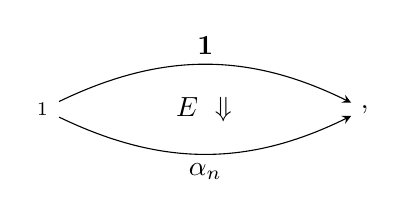
\begin{tikzpicture}[baseline=(current bounding box.center), >=stealth, scale=0.95]
  \node (A) at (0,0) {$\EBord_1$};
  \node (C) at (4.3,0) {$\Alg$,};
  \draw[->] (A) to[bend left=26] node[above] {$\mathbf 1$} (C);
  \draw[->] (A) to[bend right=26] node[below] {$\alpha_n$} (C);
  \node at (2.15,0) {$E\ \Downarrow$};
\end{tikzpicture}
\quad
\begin{array}{l@{\hspace{0.9em}}l}
E(\mathrm{pt}^{+})={}_{A}V, & E(\mathrm{pt}^{-})={}_{\ol{A}}\ol{V},\\[1pt]
E(\mathrm{I}^{+}_t)={}_{A}V\to{}_{A}V, & E(\mathrm{I}^{-}_t)={}_{\ol{A}}\ol{V}\to_{\ol{A}}\ol{V}\\[1pt]
E(\cap^{+}_t)=V\otimes_{\ol{A}}\ol{V}\to\C, & E(\cap^{-}_t)=\ol{V}\otimes_{A}V\to\C\\[1pt]
E(\cup^{+}_t)=\C\to V\otimes_{\ol{A}}\ol{V}, & E(\cup^{+}_t)=\C\to\ol{V}\otimes_{A}V\\[1pt]
E(S_t)\in V\otimes_{A\otimes\ol{A}}\ol{V} &
\end{array}
\end{array}
\tag{20}
\end{equation}
决定。翻译回定义 2.1，这引入 $\cH$ 上的一个 $A$-作用，并要求哈密顿量 $H$ 是 $A$-线性的。
% [Tutor Note: (20) 的 2-胞图中扭标作 $\alpha_n$，但本节由 (19) 定义的扭是 $\alpha_A$；(20) 正文又写 $\alpha_A$-扭场论，故图中 $\alpha_n$ 应读作 $\alpha_A$。原文如此，照排，已登记 ERRATA。]
% [Tutor Note: (20) 第四行第二个同样原写作 $E(\cup^{+}_t)$，按对称性应为 $E(\cup^{-}_t)$（与 (19) 的笔误同型）；照原样排，已登记 ERRATA。]
\end{example}

\begin{remark}[2.23]
与哈密顿量 $H$ 交换的算子是量子理论的\emph{对称性}。因此，上一个例子中 $A$-扭场论的例子也可以看作代数 $A$ 通过对称性作用的那些理论。
\end{remark}

\begin{example}[2.24（Spin 理论）]
为处理费米子（如例 2.11 那样），把配边范畴 $\EBord_1$ 加强为 $\EBord^{\mathrm{Spin}}_1$，其配边现在是带 spin 结构的欧几里得 1 维流形。spin 场论的目标范畴相应地把 $\Alg$ 加强为由 $\Z/2$-分次代数、$\Z/2$-分次双模以及保分次的双模映射构成的、带 $\Z/2$-分次张量积的双范畴。Spin 1 维流形有来自 spin 翻转的 $\Z/2$-自同构；类似地，$\Z/2$-分次代数与双模有来自其分次对合 $(-1)^{F}$ 的 $\Z/2$-自同构；见下文 (22)。更形式地说，$\EBord^{\mathrm{Spin}}_1$ 与 $\Alg$ 带有典范的 $B\Z/2$-作用。spin 场论于是是如 (11) 那样的反射正、$B\Z/2$-等变函子，而扭 spin 理论是相对于如 (20) 那样的 $B\Z/2$-等变函子的 $B\Z/2$-等变自然变换。这种 $B\Z/2$-等变性是 spin 统计定理的一个版本 [HST10, Definition 6]。

例 2.11 的自由费米子提供一个重要的例子：一个扭 spin 场论，其中 (19) 中的 $A=\mathrm{Cl}_n$ 定义扭，而 $E(\mathrm{pt}^{+})=V$ 作为 $\mathrm{Cl}_n$-模定义扭 spin 理论。半群是恒等，因此 1 维自由费米子确定一个\emph{拓扑的}扭 spin 理论。按照上一个注，$\mathrm{Cl}_n$-作用是保持作用量泛函 (9) 的经典平移对称性的量子化。要在配边框架中以正确的符号纳入这些对称性，就必须使用 spin 场论的形式体系。
% [Tutor Note: 原文此句写作 "a twisted spin field theory theory"，"theory" 重复一次；译文按单次处理，已登记 ERRATA。]
\end{example}
% [Tutor Note: 例 2.24 引用“下文 (22)”指的是 §3 中的式 (22)（$(-1)^{F}$ 的分次对合在该处正式出现），不属本块，属 sec3.tex。]
